\documentclass{article}
\usepackage[margin=1in]{geometry}
\usepackage{graphicx}
\usepackage{hyperref}
\usepackage{natbib}
\usepackage{soul}
\bibliographystyle{apalike}
\usepackage{amsmath}

\title{Fish can fly}

\author{Aden Ip$^1$\textbf{*} \and
Gledis Guri$^1$\textbf{*} \and
Ryan P. Kelly$^1$}

\date{\today}

\begin{document}

\maketitle

\section*{}

\begin{center}
\begin{tabular}{ll}
1 & School of Marine and Environmental Affairs, University of Washington, Seattle, Washington, USA \\
\hline
\textbf{*} & shared first authorship\\
&\\
& corresponding author \textbf{adenip@uw.edu}
\end{tabular}
\end{center}

\section{Introduction}
ADEN
\section{Methods}

\subsection{Sampling}
Field work details;

\subsection{Molecular work}
Wetlab work; PCR cycle conditions; qPCR machine; assays; construction of standards; etc. 


\subsection{Bayesian model}
\subsubsection{Visual observation model}
We model the upstream migration of coho salmon (\textit{Oncorhynchus kisutch}) to spawn, during which individuals accumulate at a river dam (hatchery). The hatchery crew periodically opens the dam gate at time $i$ to allow passage for spawning. Between successive gate-opening events ($\Delta i$), coho salmon gets accumulated. Let $X$ represent the true daily accumulation rate (also fish density at the river dam) in units of fish/day at time $i$, and E denote the number of days elapsed between consecutive gate openings ($ E_i =\Delta i; E_{i=1} = 0$). Prior to each gate opening, the crew conducts a visual count $N_i$ of accumulated fish.
Assuming $X_i$ remains relatively constant between successive gate-opening events ($\Delta i$), we model the observed fish counts as a Poisson process:
\begin{equation}
\lambda_i = X_i \cdot E_i \\
\end{equation}

\begin{equation}
N_i \sim \mathrm{Poisson}(\lambda_i)
\end{equation}

where, $\lambda_i$ represents the expected number of fish accumulated over the $E_i$-day interval.

\subsubsection{Molecular (water and air) observation model}
Let $W$ be the unobserved eDNA concentration (copies/$\mu$L) in the water at time $i$ and let $\omega$ be the ``integrated eDNA factor" -- the conversion factor between $X$ and $W$ (see \cite{guri2024a} for further interpretation of this parameter). We can express the relation between the fish density and water eDNA concentration as:
\begin{equation}
X_{i} = W_{i} \cdot \omega
\end{equation}

Let $A$ be the unobserved eDNA concentration (copies/$\mu$L) in the air at time $i$ that is filtered using passive filter $j$. We model the air eDNA as a function of aerosolization of the water DNA through a log-linear function with intercept $\eta$, slope = 1, and error term $\varepsilon$ (variability; time and filter specific):

\begin{equation}
\ln(A_{ij}) = \eta_{j} + \ln(W_{i}) + \varepsilon_{ij}
\end{equation}

Here the intercept $\eta$ can be interpreted as the aerosolization factor and error term $\varepsilon$ as parameter of the sum of squares error (SEE) from a linear regression where $\varepsilon_{ij} \sim \mathcal{N}(0,\tau_j)$.

For some filter types $j$ (PTFE filters (${j=P})$; gelatin filters (${j=G}$)) we had biological replicates and we used the mean of those biological replicate to determine the average concentration in the air $A$ at time $i$ as following:

\begin{equation}
%A_{ij} = \frac{1}{B} \cdot \sum_{b=1}^{B} A_{ijb}
A_{ij} = A_{ijb} + \delta_{ijb} \qquad \text{for} \ j \in \{P,G\}
\end{equation}

%\begin{equation}
%\delta_b \sim \mathcal{N}(0,\tau)
%\end{equation}

where $\delta_b$ indicates the deviation of individual biological replicate from the average concentration ($A_{ij}$), following a normal distribution with mean 0, $\delta_{ijb} \sim \mathcal{N}(0,\rho_j)$, with $\rho_j$ indicating the magnitude of the replicates deviation from the mean sample. Because we have only two replicates at each sampled time, we impose a sum to zero constraint on the replicates ($b$) collected from a single sampling time ($\sum_b \delta_{ij} = 0$).

To estimate the levels of eDNA concentration in water ($W$) and air ($A$) we make use of the qPCR observation models (as described in \cite{guri2024, shelton2022}, with slight modifications). The model compartment use the standard samples to estimate the intercept ($\phi,\beta0,\gamma0$) and slope ($\beta1, \gamma1$) parameters between the known concentration ($K$) and the observed data ($Z$ and $Y$) from qPCR machine as follow:

\begin{align}
    Z_{kr} &\sim \mathrm{Bernoulli} \left(\psi_{k}\right)  \\
    \psi_{k} &= 1 - \exp(-K_{k} \cdot \phi) \\
    Y_{kr} &\sim \mathrm{Normal} (\mu_{k}, \sigma_{k}) \quad \text{if } Z_{kr} = 1 \\
    \mu_{k} &= \beta_0 + \beta_{1p} \cdot \ln (K_{k}) \\
    \sigma_{k} &= \exp(\gamma_0 + \gamma_1 \cdot \ln (K_{k}))
\end{align}

where $Z$ is the binary outcome for sample ($k$) and technical replicate ($r$) being present (1) or absent (0) following a Bernoulli distribution given the probability of detection $\psi$ for each sample ($k$). The parameter $\phi$ is the intercept of the function between probability of detection $\psi$ and the known DNA concentration ($K$; copies/$\mu$L) as the predictor variable. Additionally, for equations 8-10, $Y$ is the observed cycle threshold (Ct) for sample ($k$) and technical replicate ($r$) which follows a normal distribution with mean $\mu$ (mean Ct) and standard deviation $\sigma$ for each sample ($k$). We model $\mu$ as a linear function of known eDNA concentration ($K$) with intercept $\beta0$ and slope $\beta1$ and the standard deviation $\sigma$ of the observed Y as an exponential function of known eDNA concentration with intercept $\gamma0$ and slope $\gamma1$.

Subsequently we build the same model compartment for estimating eDNA concentration in water ($W$) and air ($A$) by substituting $W_i$ and $A_{ij}$ (and $A_{ijb}$ for $j \in \{P,G\}$) respectively with $K_k$ through equation 6-10 (see DAG) where intercept and slope parameters between DNA concentration and qPCR observation are shared between model compartments.

\subsection{Model conditions}
The joint model (DAG XXX) was implemented using the Stan language as implemented in R (package: Rstan) running four independent MCMC chains using 4000 XXX warmup and 6000 XXX sampling iterations (Table XXX for parameters and their priors). The posterior predictions were diagnosed using statistics (Gelman and Rubin 1992) and considered convergence for values less than 1.05 and effective sample size (ESS) greater than 1000 for all parameters.

\begin{figure}[tbhp] 
\centering
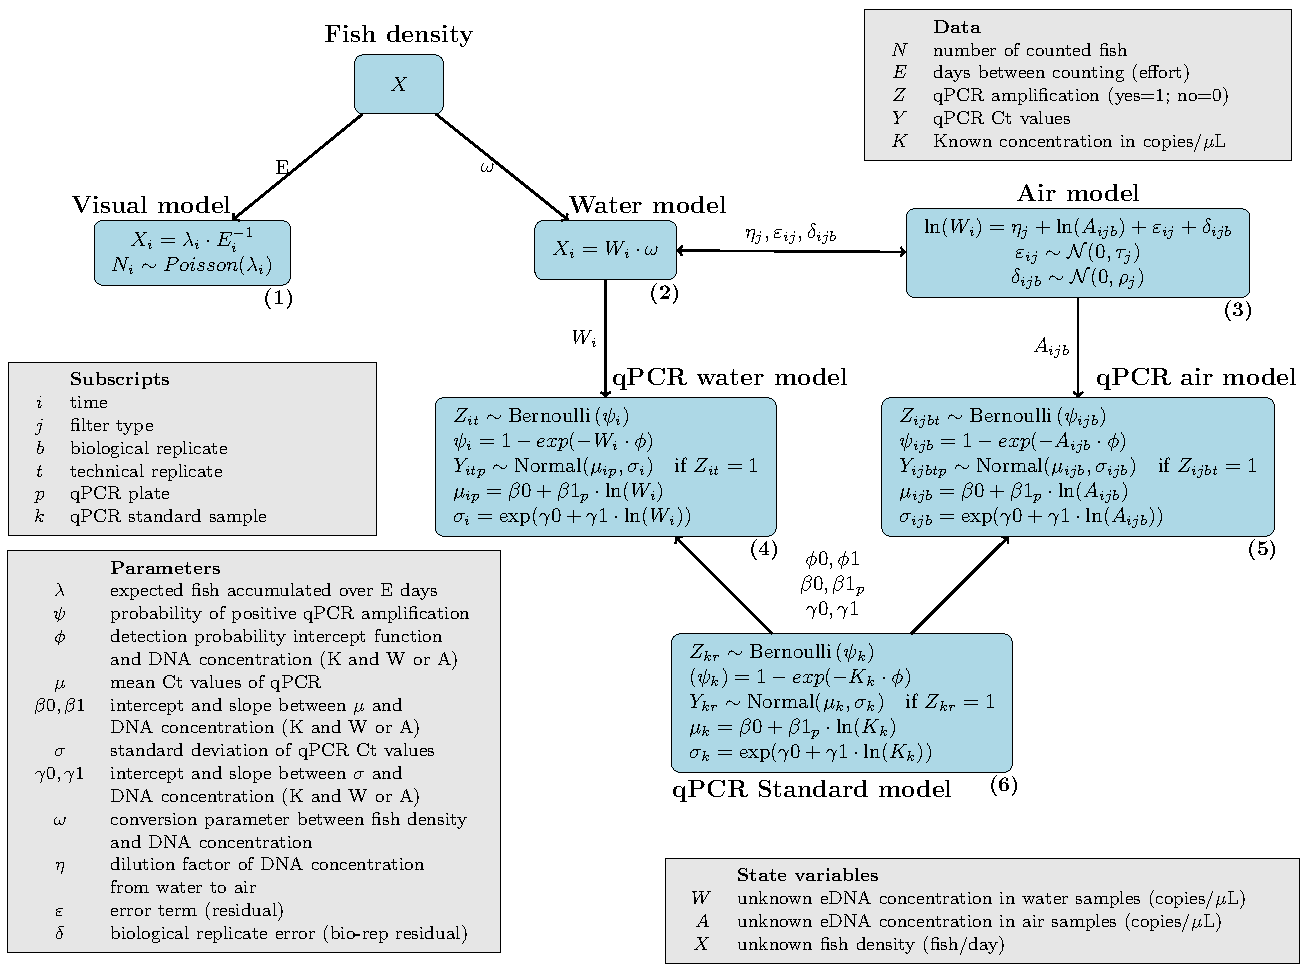
\includegraphics[width=16.5cm]{Plots/DAG.pdf}  
\caption{Correlation plot describing species co-abundance and co-occurance. Spearman’s $\rho$ correlation coefficient are expressed in numbers and colors ranging from -1 (red) negatively correlated to 1 (blue) positively correlated. Species are ordered in known ecological groups (surface, midwater, and deepwater) to visually indicate the gradual change of species co-occurance.}
\label{fig:DAG}
\end{figure}

\section{Results}

\begin{figure}[tbhp] 
\centering
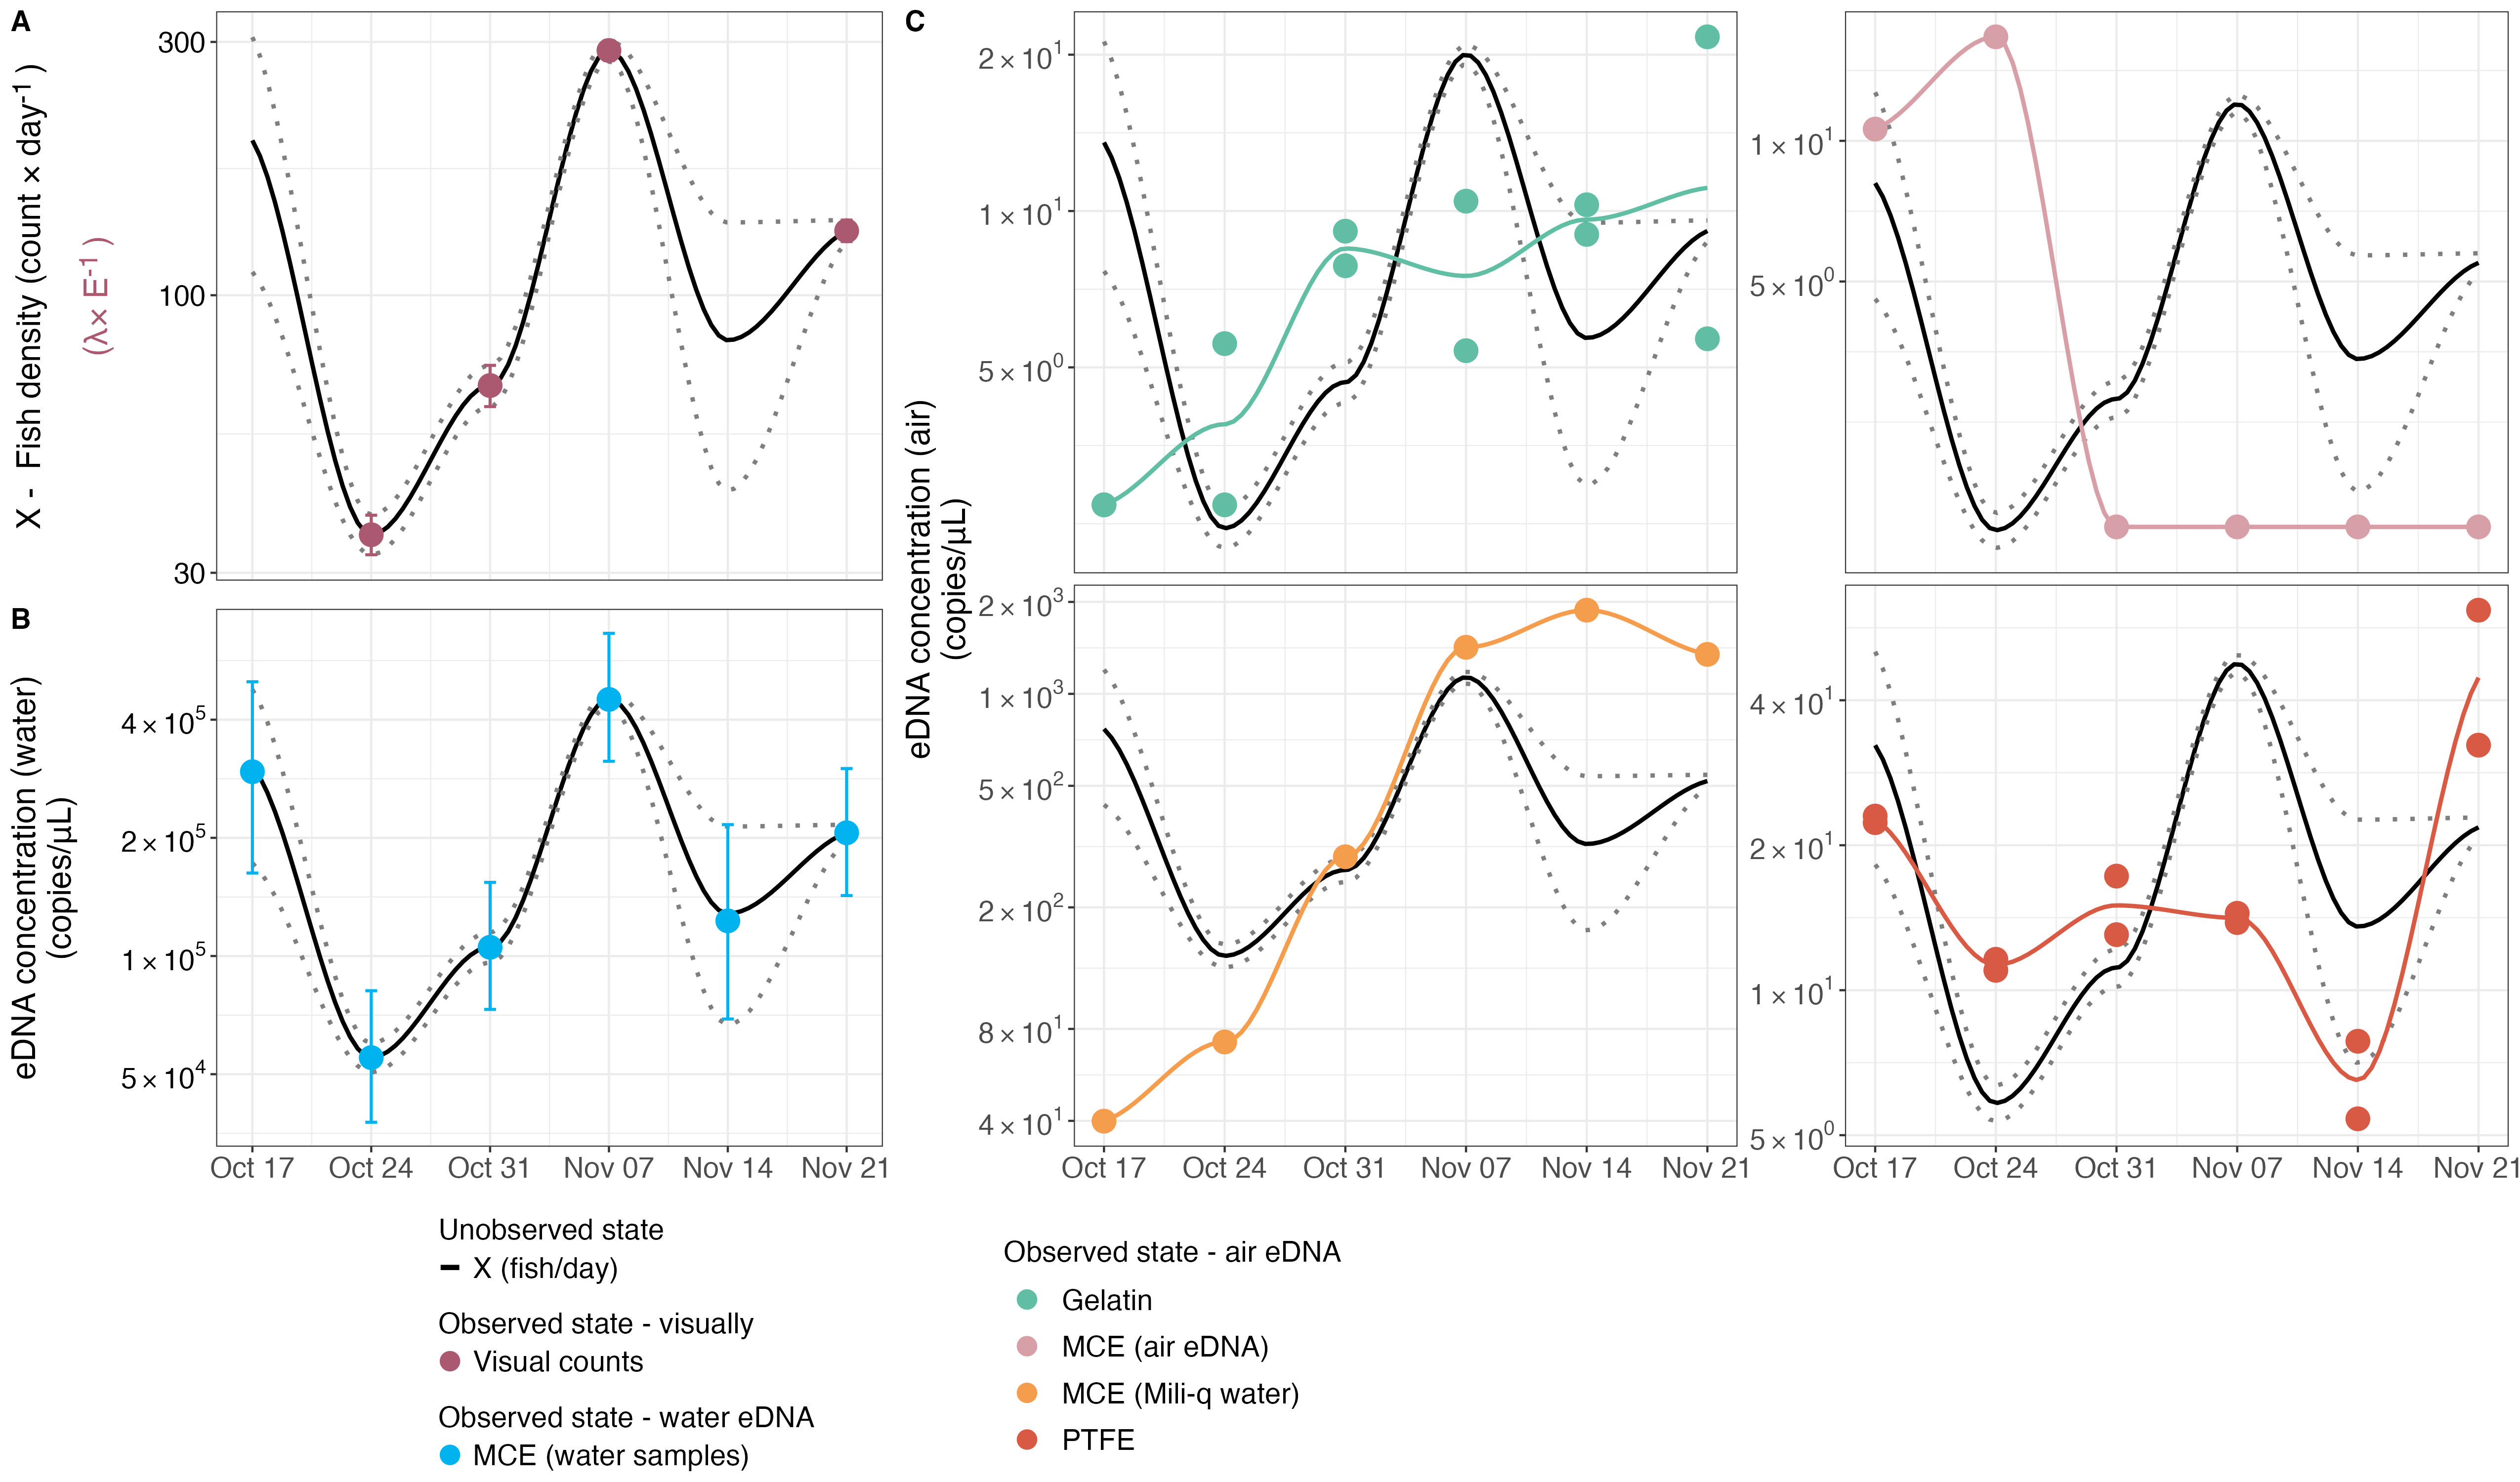
\includegraphics[width=18cm]{Plots/Figure_1.jpg}  
\caption{Correlation plot describing species co-abundance and co-occurance. Spearman’s $\rho$ correlation coefficient are expressed in numbers and colors ranging from -1 (red) negatively correlated to 1 (blue) positively correlated. Species are ordered in known ecological groups (surface, midwater, and deepwater) to visually indicate the gradual change of species co-occurance.}
\label{fig:fig1}
\end{figure}


\begin{table}[h!]
\centering
\caption{Error measurements for different filter types}
\label{tab:filter_error}

\begin{tabular}{llll}
\textbf{Filter type} & \textbf{Dilution ($\eta$)} & \textbf{Error ($\overline{|\varepsilon|}$)} & \textbf{Biological rep error ($\overline{|\delta|}$)} \\
Gelatin & $e^{-9.25}$ & 0.788 & 0.230 \\
PTFE & $e^{-8.39}$ & 0.570 & 0.106 \\
MCE Air & $e^{-9.77}$ & 1.370 & - \\
MCE DI water & $e^{-5.33}$ & 0.974 & - \\
\end{tabular}
\end{table}

\bibliography{Bib.bib}
\end{document}


\begin{table}[h]
    \centering
    \begin{tabular}{llll}
        \textbf{Filter type} & \textbf{Dilution ($\eta$)} & \textbf{Error ($\overline\varepsilon$)} & \textbf{Biological rep error ($\overline\delta$)} \\
        Gelatin & $e^{-9.5}$ & 0.628 & 1.315 \\
        PTFE & $e^{-8.8}$ & 0.666 & 0.682 \\
        MCE air filter & $e^{-10.2}$ & 1.133 & - \\
        DI water & $e^{-5.7}$ & 0.606 & - \\
    \end{tabular}
    \caption{Error measurements for different filter types}
    \label{tab:filter_error}
\end{table}



Fish Density Model (Water): The number of fish counted ('N') at a given point is assumed to be proportional to the total amount of water-borne DNA, which can be estimated from measurements taken underwater and converted into an 'eDNA concentration' parameter ('W'). This conversion process involves multiplying by another factor called 'omega', denoted as 'ω'.
Air Model: The eDNA concentrations in air samples are calculated based on those found in the corresponding water sample using a dilution factor, which is determined from measurements taken underwater and above ground (i.e., atmospheric pressure). These factors include both known ('K') and unknown values of DNA concentration that need to be estimated during model fitting or inference processes.
qPCR Model: The number of positive amplification results in the various types of samples are assumed to follow a Poisson distribution, with mean proportional to their respective eDNA concentrations (W for water-borne species) as well as effort ('E', which represents days between counting). This relationship is captured by parameters like 'phi0' and 'phi1'.
Visual Model: The probability of finding fish in an underwater visual census survey follows a logistic model, with the logit link being determined by linear combinations involving eDNA concentration (W) as well as other covariates ('X') such as depth or temperature measurements taken at each counting event. This relationship is represented by parameters like 'beta0' and 'beta1'.
Standard Model: In cases where a known standard sample with DNA content of K copies/μL exists, the model allows for estimation of eDNA concentrations in water samples ('W') using this reference value as well as other covariates (X). The relationship is determined by parameters like 'gamma0' and 'gamma1'.
Error Terms: Various error terms are included to account for uncertainty or variability introduced during different stages of the analysis process, such as biological replicates in air sampling ('delta b'), residuals from model equations involving eDNA concentration (omega), dilution factors between water-borne vs atmospheric DNA samples (eta) and technical replicate measurements taken within each type of sample. By incorporating these relationships into a single graphical structure that can be analyzed using statistical software, researchers are able to estimate parameters like 'W', 'A' or other key ecological variables with improved accuracy compared to traditional methods relying solely on one specific analytical technique alone (e.g., qPCR).

We can start by defining λ as fish density, where ω represents a conversion parameter from fish/day to copies/μL (the unit for DNA concentrations). This means that W = λ * ω and $A_b = η^(-1)$ / B. The air model also includes the δ error term representing biological replicate differences between samples taken at different times or using different filters, leading to a final equation of:
Aij= (ηj + ln(PB))/B with PB being an unknown constant that depends on both filter type and bioreplicate difference in time. The qPCR water model can be defined similarly as $Z = ψ_i * W^(-1)$ where μ is the mean Ct values of a standard curve, β represents slopes between DNA concentration (K or A), σ being its corresponding error term for each sample i at different times t during counting and plate p. The qPCR air model can be defined as $Z = ψ_k * K^(-1)$ with μ representing the mean Ct values of a standard curve, β represents slopes between DNA concentration (K or A), σ being its corresponding error term for each sample i at different times t during counting and plate p. The qPCR Standard model can be defined as $Z = ψ_i * W^(-1)$ with φ representing intercepts/slopes of the probability response to standard curve concentrations K, μ mean Ct values from a single amplification cycle (Ct), σ being its corresponding error term for each sample i at different times t during counting and plate p. The parameters can be estimated using maximum likelihood estimation or Bayesian methods such as MCMC sampling if needed given prior distributions specified on all unknown quantities including $W_i = η^(-1) / B$ with PB representing an unknown constant that depends both filter type bioreplicate difference in time, ε error term (residual), and δ being biological replicate errors. The subscripts provide information about the variables at different times i during counting or using filters jb for each sample b taken over multiple plates pqPCR standard samples k
